\documentclass[11pt,a4paper]{article}
\usepackage[margin=0.8in]{geometry}
\usepackage[T1]{fontenc}
\usepackage[utf8]{inputenc}
\usepackage{lmodern}
\usepackage{amsmath,amssymb}
\usepackage{graphicx}
\usepackage{caption}
\usepackage{booktabs}
\usepackage{longtable}
\usepackage{tabularx}
\usepackage{enumitem}
\usepackage{hyperref}
\usepackage{xcolor}

% Custom Colors for a professional look
\definecolor{aybu_blue}{RGB}{31, 73, 125}
\definecolor{section_gray}{RGB}{242, 242, 242}

\hypersetup{
    colorlinks=true,
    linkcolor=aybu_blue,
    urlcolor=blue
}

\graphicspath{{./diagrams_aybustore/}}

\title{\LARGE \textbf{AYBUStore: Intelligent Campus E-Commerce Ecosystem}\\[0.5em] \large Supplementary Technical Report for TÜBİTAK 1001 Proposal}
\author{Utkan Dindaroğlu, Seyfullah Gülyazı, Süleyman Fatih Sert, Ahmet Selim Yılmaz, Muhammed Yıldız}
\date{\today}

\begin{document}

\maketitle

\begin{abstract}
This report details the technical architecture, methodology, and requirement specifications for AYBUStore, a smart e-commerce platform developed for Ankara Yıldırım Beyazıt University. Utilizing a modern stack of Next.js 14 and Firebase, the project integrates AI-driven personalization and real-time inventory management to solve physical campus commerce inefficiencies.
\end{abstract}

\section{Introduction \& Problem Definition}
The AYBUStore project addresses the lack of a centralized digital ecosystem for university-branded merchandise and department-specific materials. Existing solutions fail to provide real-time stock transparency, personalized apparel preview, or AI-integrated shopping assistance.

\subsection{Scientific Excellence: Hyper-Local Closed-Loop Digital Ecosystem}
As detailed by the research team (U. Dindaroğlu), the project conceptualizes a \textbf{Hyper-Local Closed-Loop Digital Ecosystem (HL-CLDE)} specifically tailored for a distributed university environment. Unlike standard e-commerce platforms, AYBUStore addresses the \textit{Four-Campus Distribution Problem} where geographical fragmentation between Esenboğa, Etlik, Bilkent, and Çubuk campuses limits brand physical accessibility. By digitizing inventory and centralizing logistics, the platform targets a \textbf{30\% increase in merchandise accessibility} for students. A core focus is the optimization of \textbf{Time-to-Interactive (TTI)}, aiming for a \textbf{1.2s benchmark} to ensure seamless user engagement across varied campus network conditions.

\section{System Architecture}
We adopt a \textbf{Component-Based Architecture} using Next.js App Router for optimal performance and SEO. The backend is powered by Firebase, providing a serverless real-time database and secure authentication.

\subsection{Use Case Analysis}
The following diagram illustrates the interactions between students, staff, and administrators within the ecosystem.

\begin{center}
    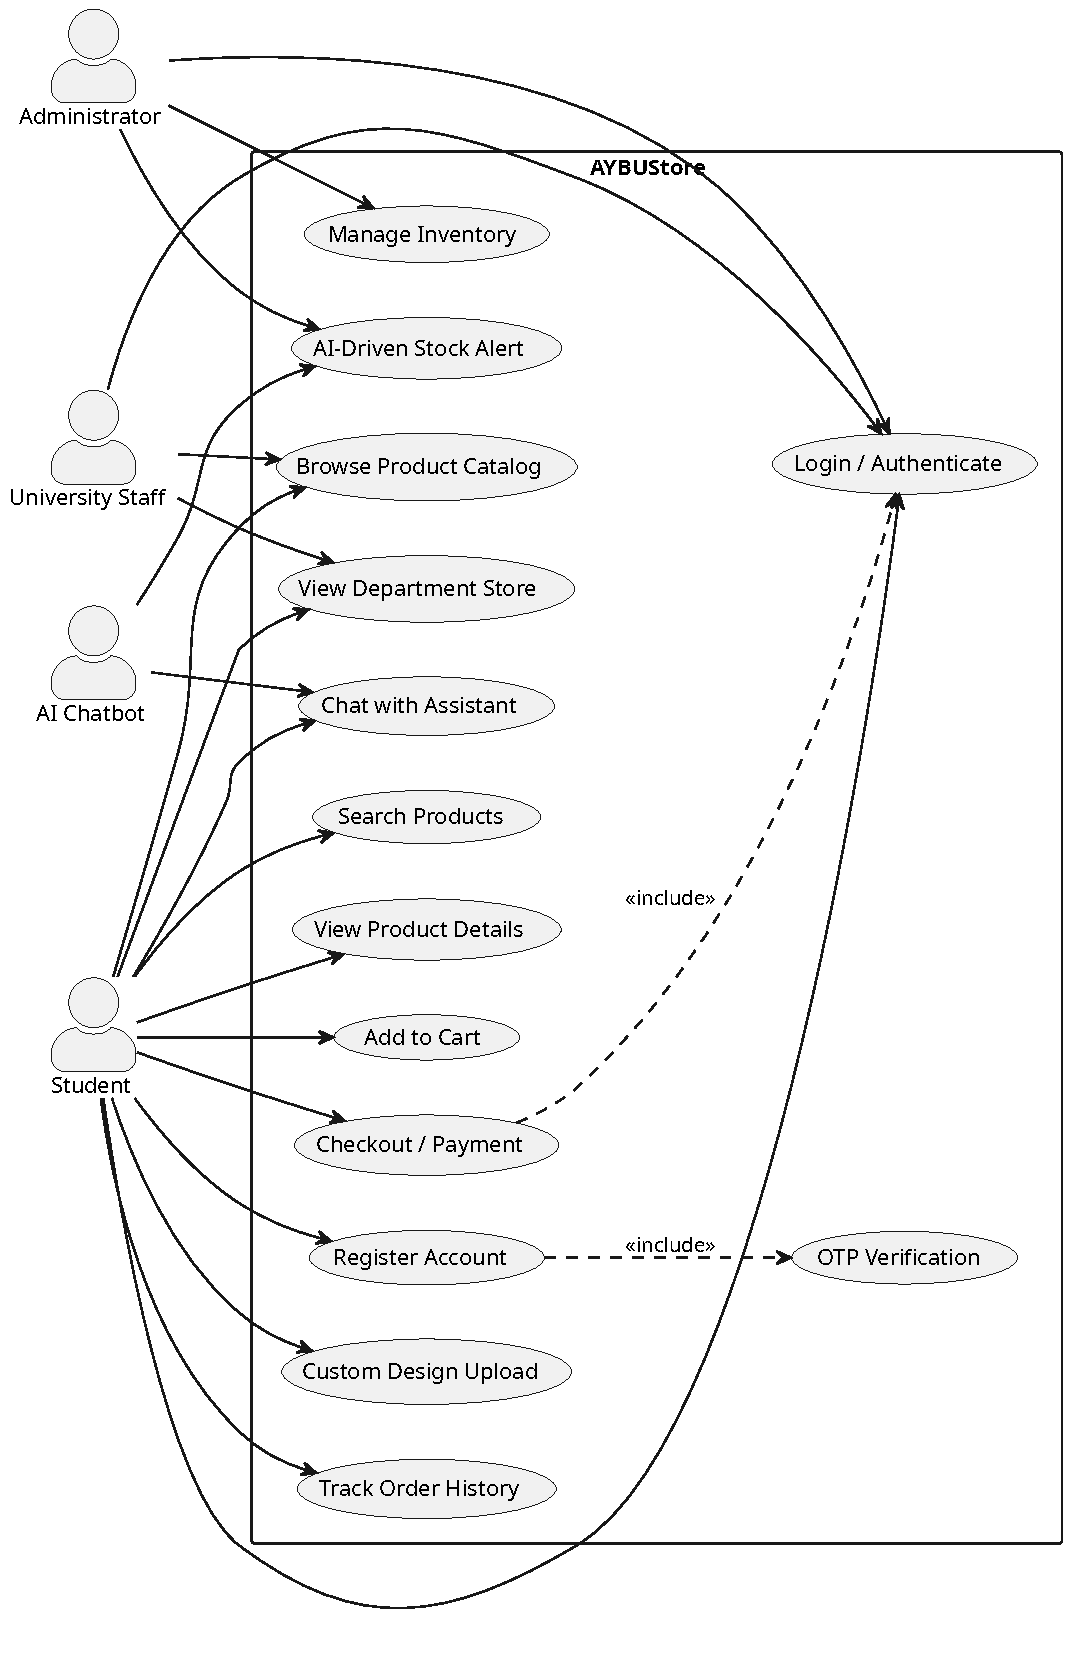
\includegraphics[width=0.8\textwidth]{use_case_diagram}
    \captionof{figure}{AYBUStore Use Case Diagram (Vector)}
\end{center}

\subsection{Domain Modeling}
The system's data structure is designed with modularity in mind, ensuring scalability as new faculties are added.

\begin{center}
    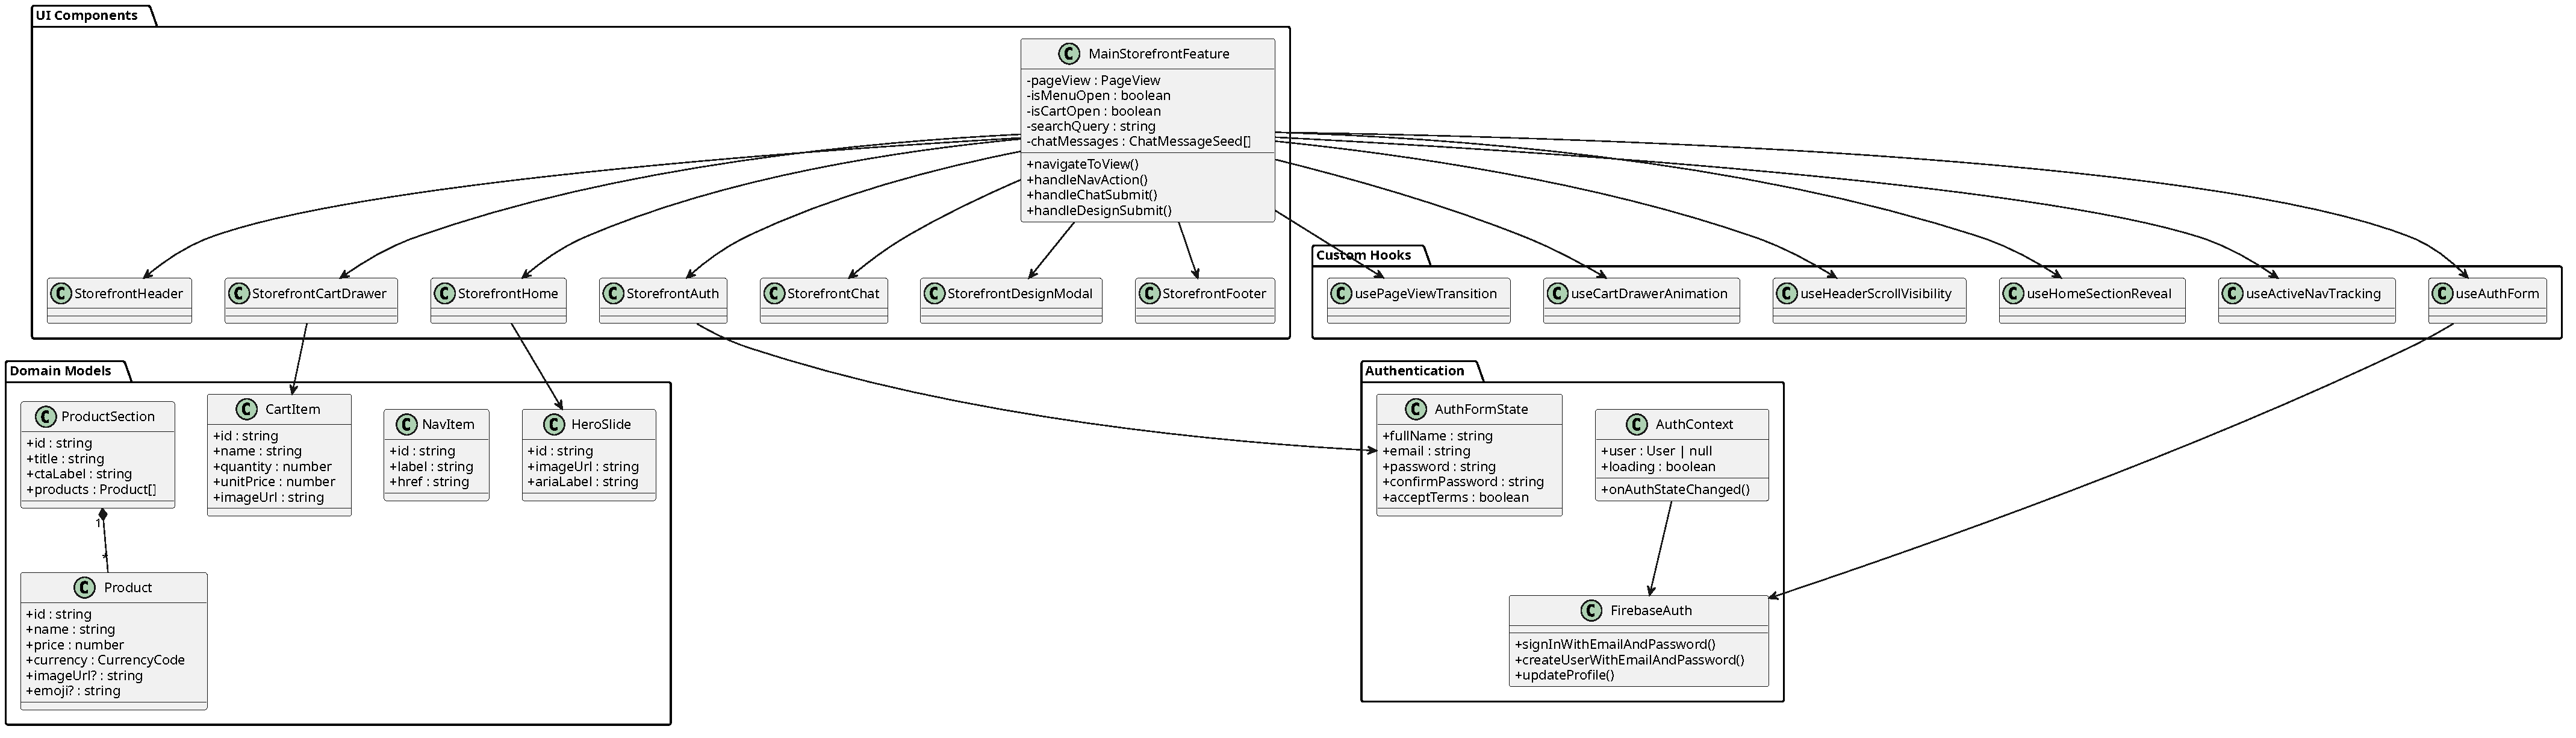
\includegraphics[width=0.9\textwidth]{class_diagram}
    \captionof{figure}{System Domain Class Diagram}
\end{center}

\section{Core Processes}
\subsection{Authentication \& OTP Flow}
Security is managed via a multi-stage authentication process, verified by a 6-digit one-time password (OTP) sent to university emails.

\begin{center}
    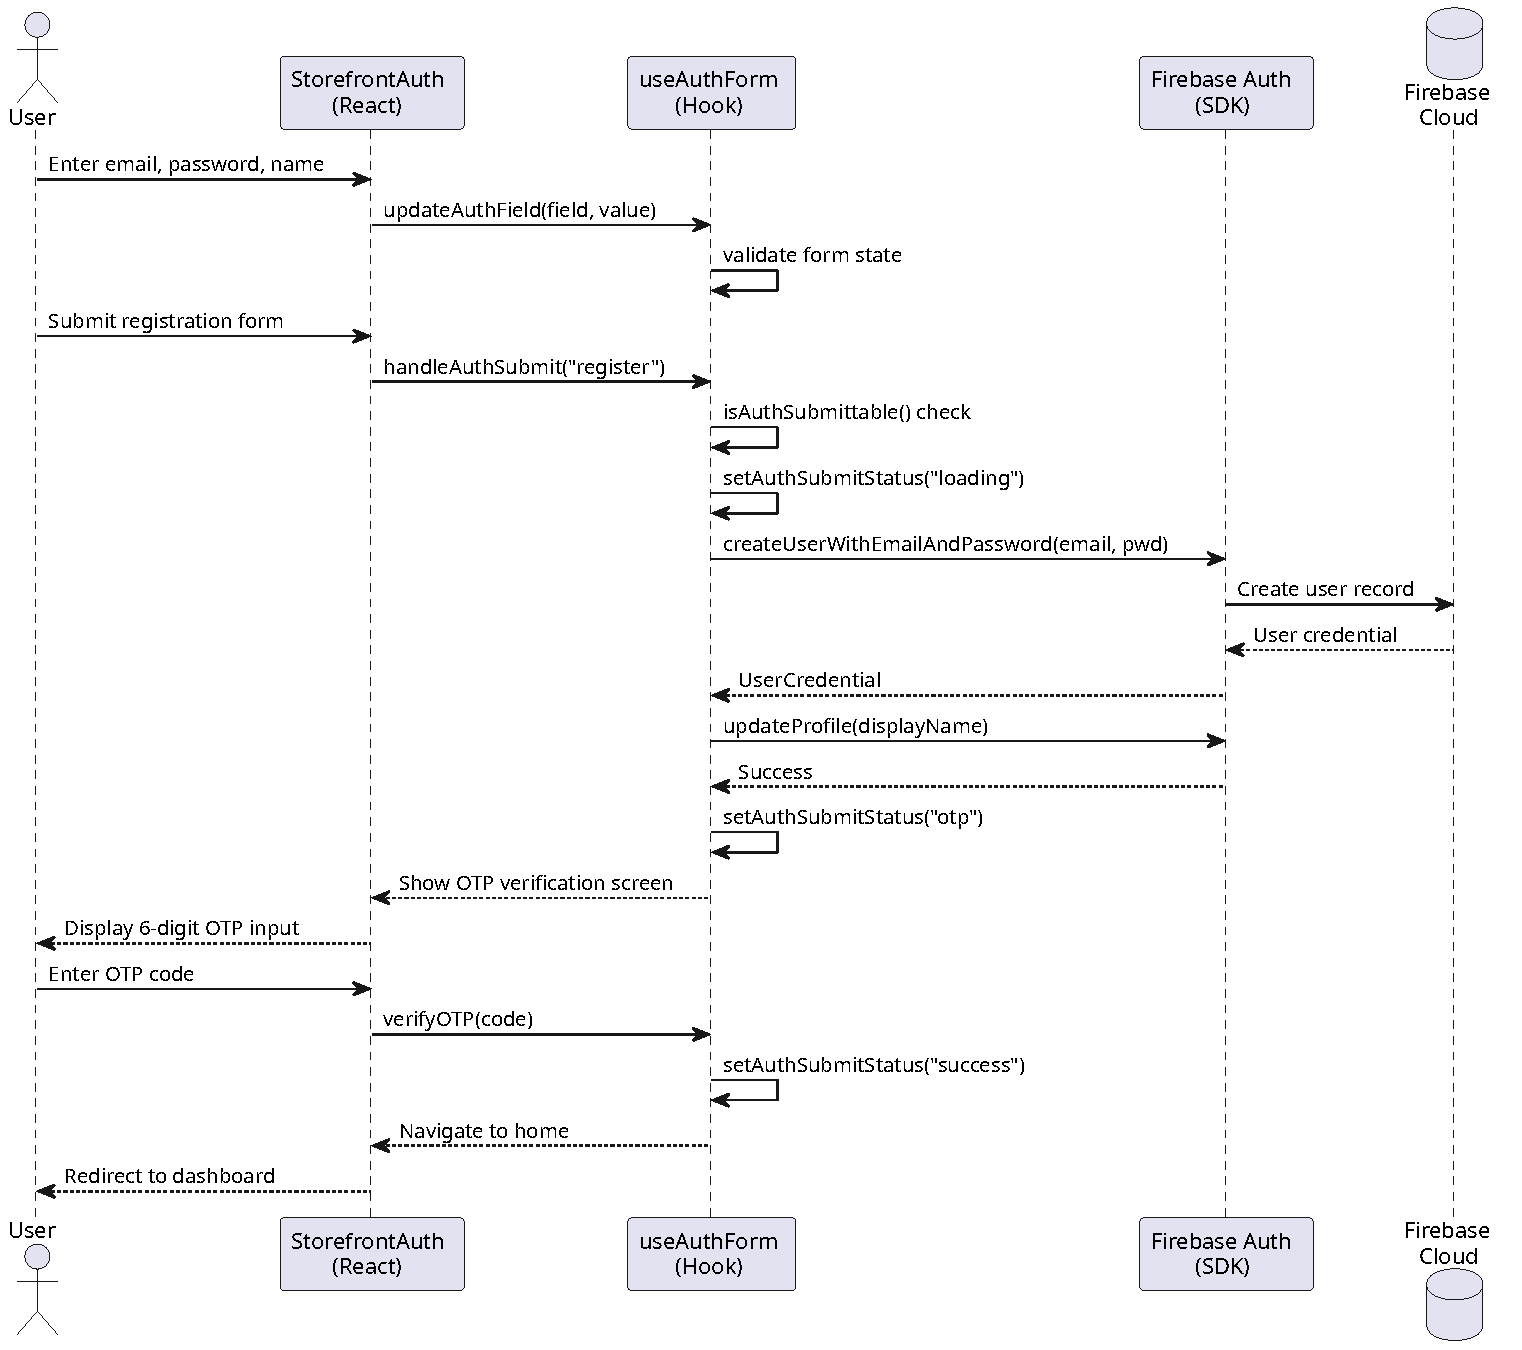
\includegraphics[width=0.8\textwidth]{sequence_auth}
    \captionof{figure}{Registration and Security Verification Sequence}
\end{center}

\subsection{AI Personalization}
The AI Shopping Assistant utilizes LLM-based intent analysis to provide context-aware product recommendations.

\begin{center}
    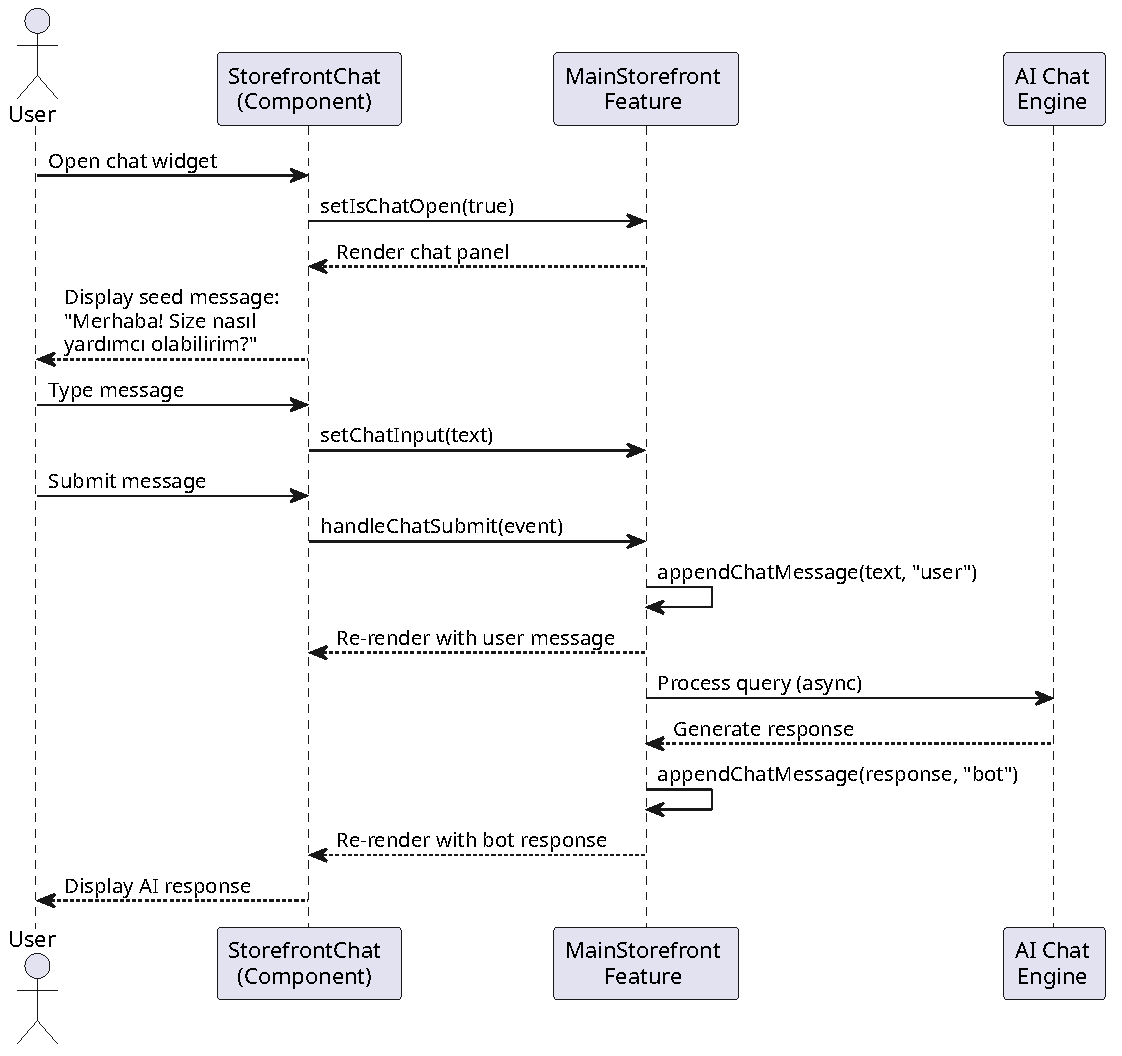
\includegraphics[width=0.8\textwidth]{sequence_chat}
    \captionof{figure}{AI-Driven Assistant Interaction Flow}
\end{center}

\section{Operational Design}
\subsection{Shopping Lifecycle}
The activity flow below describes the transition from browsing to custom design and final checkout.

\begin{center}
    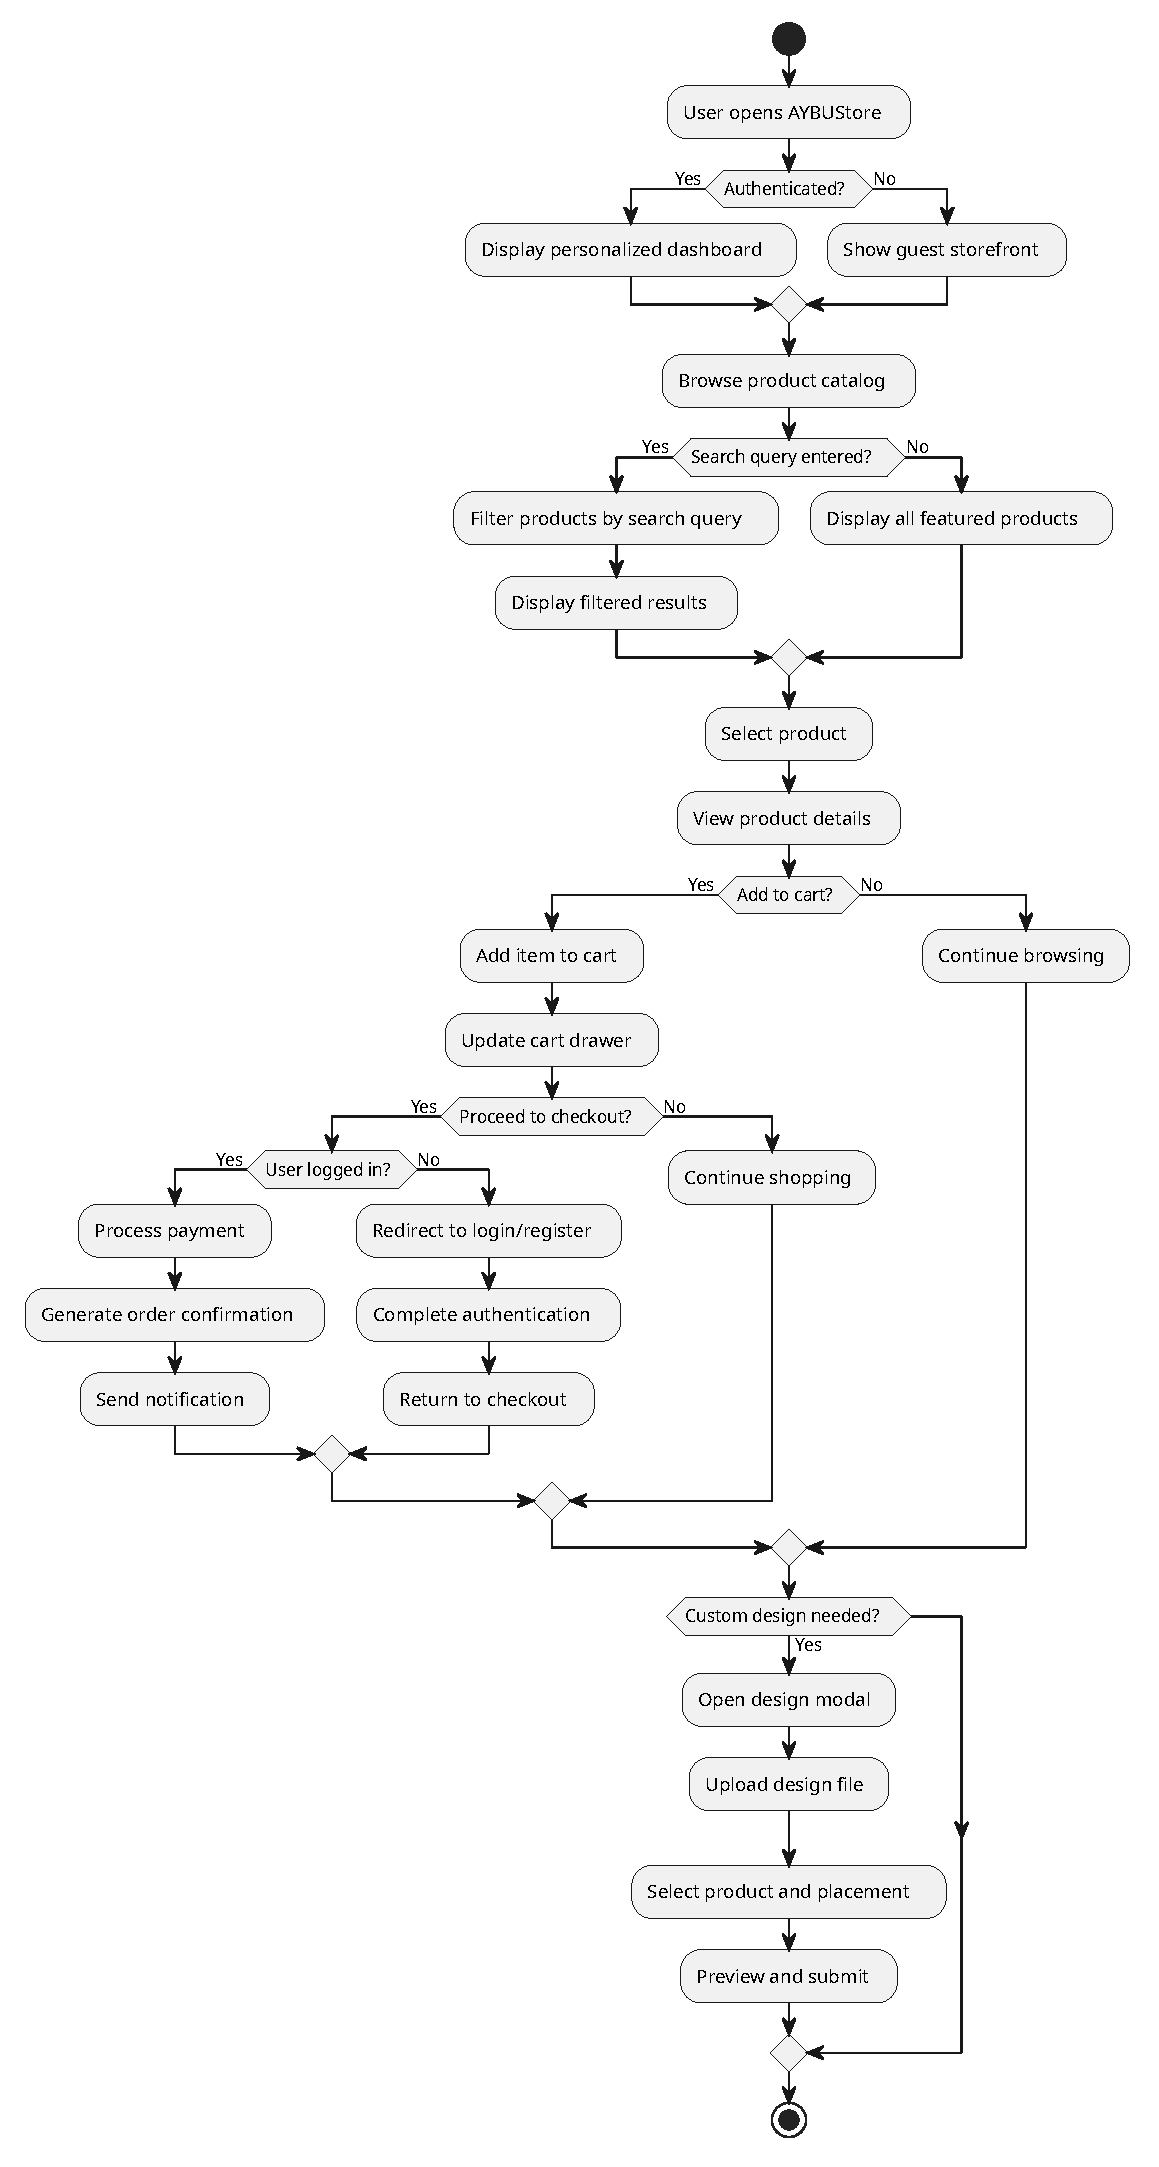
\includegraphics[width=0.8\textwidth]{activity_diagram}
    \captionof{figure}{User Activity Lifecycle Diagram}
\end{center}

\section{Methodology \& Software Requirement Specification}
\subsection{The 5-Phase Iterative Process}
The development lifecycle follows a structured 5-phase iterative process as designed by A.S. Yılmaz:
\begin{itemize}
    \item \textbf{Phase 1: Domain-Driven Design (DDD) Paradigm} - Mapping complex campus operations into bounded contexts (Authentication, Storefront, and Logistics).
    \item \textbf{Phase 2: Architectural Justification} - Selecting Node.js/Next.js over traditional Spring Boot or Python frameworks for superior non-blocking I/O and server-side rendering (SSR) capabilities.
    \item \textbf{Phase 3: Shift-Left Validation} - Integrating continuous testing and linting from the first commit to ensure code quality and prevent technical debt.
    \item \textbf{Phase 4: Work Package Distribution} - Execution of five specific work packages: WP1 (Core Infrastructure), WP2 (Secure Auth), WP3 (Dynamic Storefront), WP4 (AI \& Logistics), and WP5 (User Acceptance).
    \item \textbf{Phase 5: Logistics and Notification Pipeline} - Finalizing the real-time notification system for order status transitions.
\end{itemize}

\subsection{Risk Management}
\begin{table}[h]
\centering
\begin{tabularx}{\textwidth}{@{}lXXl@{}}
\toprule
\textbf{Risk ID} & \textbf{Identified Risk} & \textbf{Mitigation Strategy} & \textbf{Impact} \\ \midrule
R1 & AI Query Hallucination & Prompt engineering and context-window constraints. & Medium \\
R2 & Multi-campus Latency & CDN edge caching and optimized TTI benchmarks (1.2s). & High \\
R3 & Firebase Data Scale & Implementing optimized Firestore indexing and sharding. & Low \\
R4 & Authentication Bypass & Multi-stage OTP verification and secure AuthContext. & Critical \\ \bottomrule
\end{tabularx}
\caption{Project Risk Assessment and Mitigation Matrix}
\end{table}

\subsection{Software Requirement Specification (SRS)}
\textbf{Functional Requirements (FR):}
\begin{enumerate}
    \item User registration with university email verification.
    \item Secure 6-digit OTP-based authentication flow.
    \item Dynamic product catalog with category-based filtering.
    \item Real-time inventory tracking and stock status display.
    \item AI-powered shopping assistant for product inquiries.
    \item "Design Your Own" custom merchandise preview module.
    \item Persistent shopping cart management and state recovery.
    \item Real-time order status tracking and logistics notifications.
    \item Administrative CMS panel for product and user management.
    \item Multi-campus logistics routing for Etlik, Bilkent, Esenboğa.
\end{enumerate}

\textbf{Non-Functional Requirements (NFR):}
\begin{enumerate}
    \item \textbf{Performance:} Time-to-Interactive (TTI) must be less than 1.2s on campus networks.
    \item \textbf{Scalability:} Support up to 5,000 concurrent student users during peak periods.
    \item \textbf{Security:} SSL encryption for all data in transit and Firebase Security Rules for DB.
    \item \textbf{Responsiveness:} Fully adaptive UI for mobile, tablet, and desktop viewports.
    \item \textbf{Availability:} 99.9\% system uptime via serverless Vercel/Firebase infrastructure.
\end{enumerate}

\section{Team, Resource Plan \& Cost Estimation}
\subsection{Git-Based Contribution Audit}
Based on the audit of the \texttt{muhammed\_latest\_patch} branch, the following roles are assigned:
\begin{itemize}
    \item \textbf{Muhammed Yıldız (Core Architect):} Established project infrastructure, Firebase Auth, CI/CD pipelines, and core state management (AuthContext).
    \item \textbf{Utkan Dindaroğlu (Scientific Research):} Led the modular refactoring, advanced UX animations, and HL-CLDE ecosystem design.
    \item \textbf{Ahmet Selim Yılmaz (Process Design):} Defined the 5-phase methodology and SRS alignment with university standards.
    \item \textbf{Seyfullah Gülyazı \& S. Fatih Sert (Implementation):} Managed specialized UI components and the logistics notification engine integration.
\end{itemize}

\subsection{COCOMO Cost Estimation}
Calculated using the \textbf{Organic Mode} for a team-driven academic project:
\begin{itemize}
    \item \textbf{Estimated KLOC:} 2.69 (Actual repository audit).
    \item \textbf{Effort Equation:} $E = 2.4 \times (KLOC)^{1.05}$.
    \item \textbf{Result:} $E \approx 6.8$ Person-Months.
    \item \textbf{Schedule:} $T = 2.5 \times (E)^{0.38} \approx 5.2$ Months for total project completion.
\end{itemize}

\section{Conclusion}
AYBUStore provides a scalable and intelligent solution for campus commerce, leveraging modern web technologies to enhance the university's digital brand.

\end{document}
